% \begin{figure}[h!] 
	\centering
	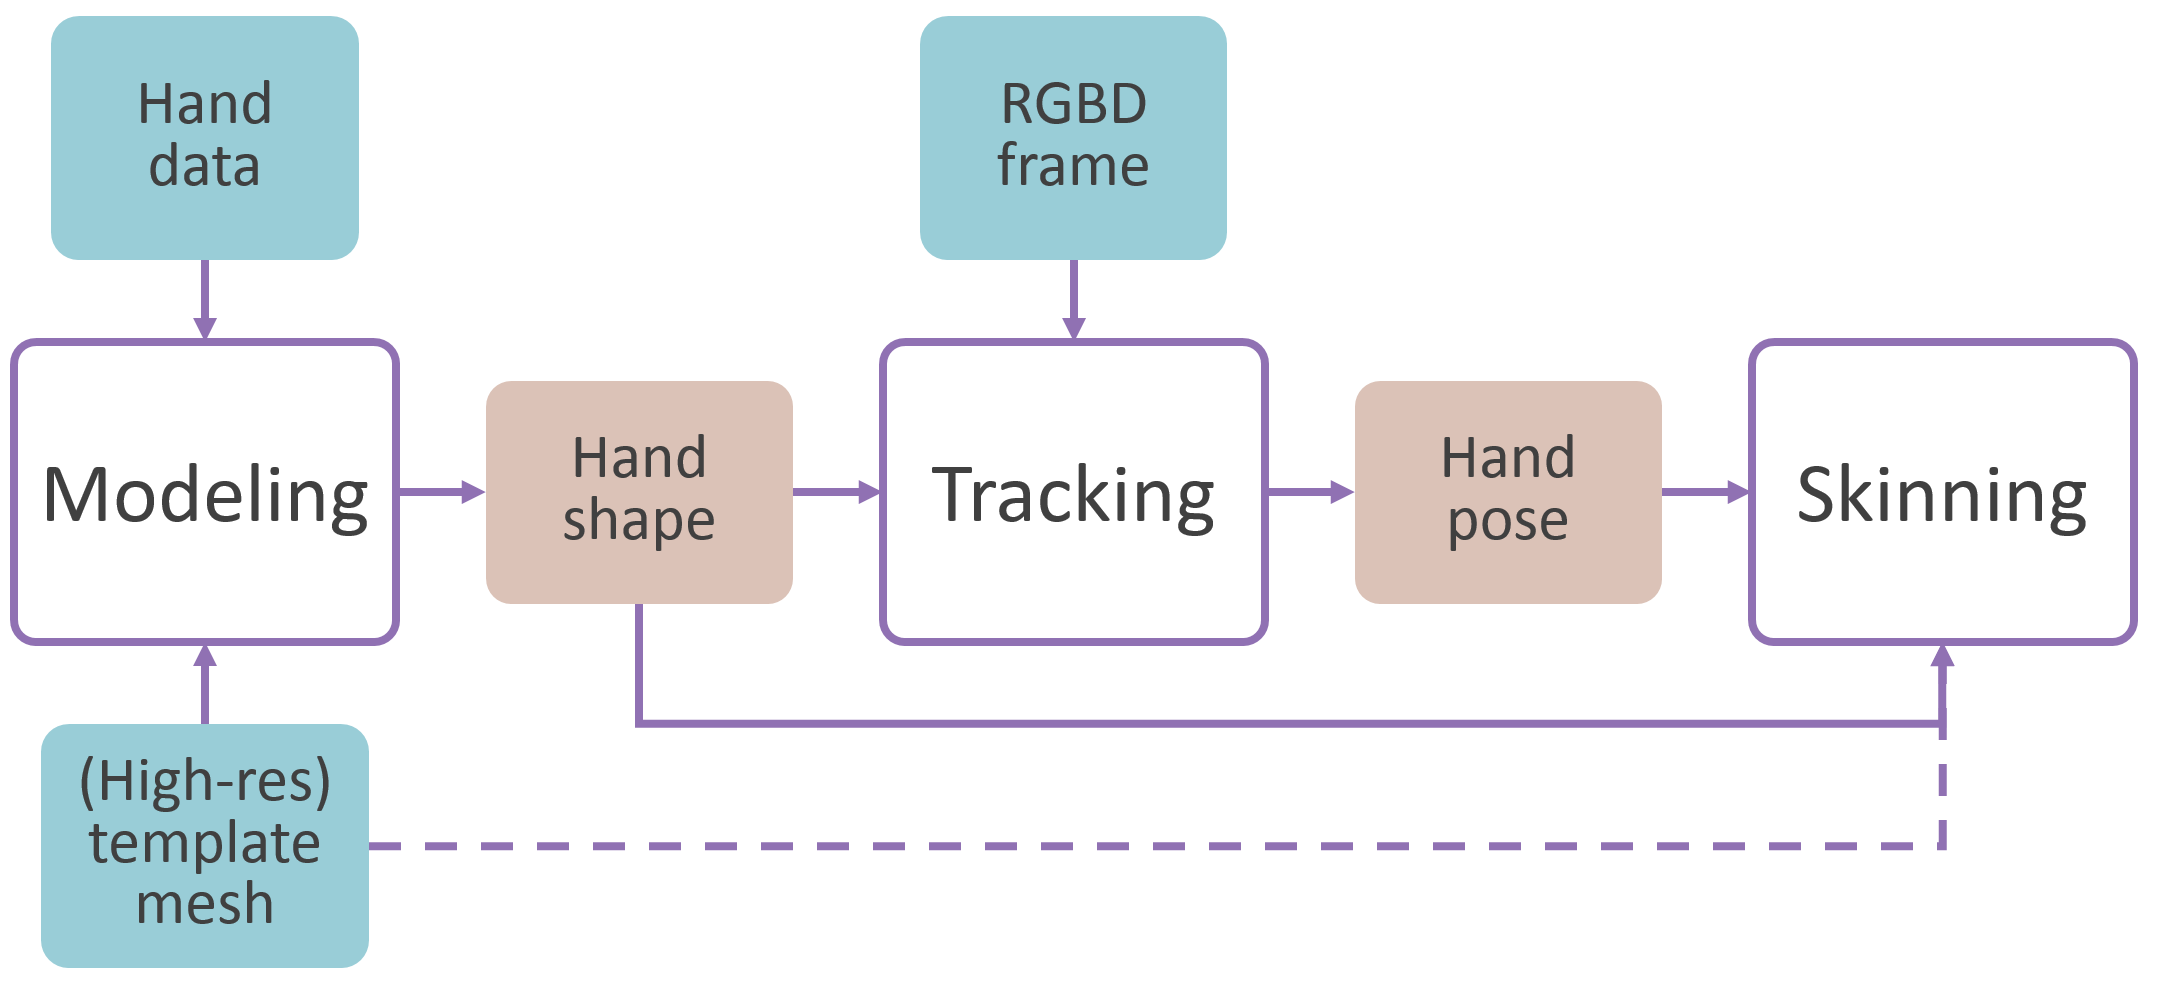
\includegraphics[width=0.5\textwidth]{fig/generic_pipeline}
	\caption{Generic pipeline for hand tracking. The input data that does not depend on the internal hand model representation is shown in blue, the representation-dependent components are shown in beige, and are listed in Table \ref{table:representation_dependent_components} for different representations.}
	\label{fig:generic_pipeline}
\end{figure} %<<< TO REMOVE!

The triangles mesh representation can approximate the hand to a high precision. However, it is not trivial to specify the model parts that are rigid and should be kept the same shape between the poses. This results in overfitting to local skin deformations. 

However, in most consumer applications hand tracking is just a single components of a bigger pipeline (Figure \ref{fig:generic_pipeline}). Before tracking, a suitable hand model is obtained. Once the hand pose parameters are found, the tracking result is displayed by skinning the model. Both modeling and skinning tasks are not trivial.

\begin{figure}[h!] 
\centering
\hspace{-2em}
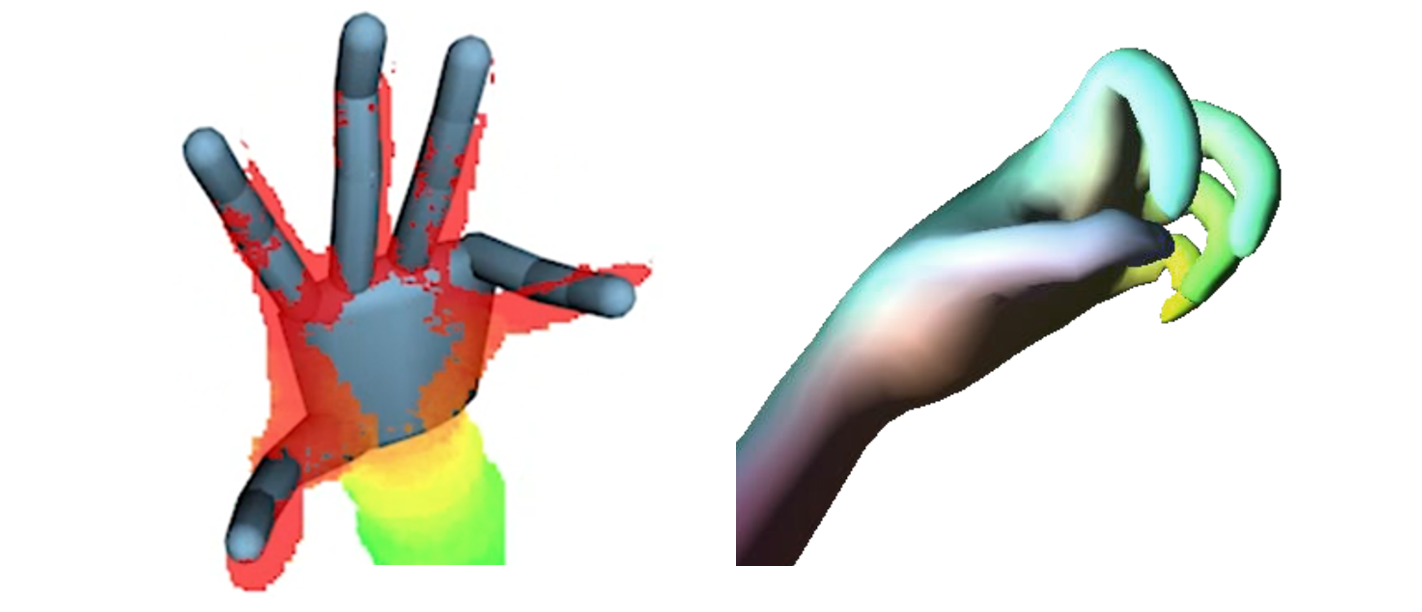
\includegraphics[width=0.5\textwidth]{fig/coarse_hand_model_and_lbs}
\caption{}.
\label{fig:coarse_hand_model_and_lbs}
\end{figure}

Especially if the hand model does not reflect all the degrees of freedom of a hand (Figure \ref{fig:coarse_hand_model_and_lbs}, left).

Each stage of the pipeline requires a hand model. There is several different hand model representations suggested by previous authors (see Figure \ref{fig:hand_model_representations}). Each representation is well suited for one of the stages, since it was used for the task on the first place. We argue that each representation also has weaknesses, which is why there exists a set of alternatives.

%--- OLD CONVOLUTION SURFACES TEXT
We suggest to use convolution surfaces representation of the hand model. Convolution surface is an implicit surface which is described by a control skeleton. The skeleton may consist of points, edges or polygons \cite{bloomenthal1991convolution}. In each vertex of the skeleton we define a radius. The radius in intermediate points is a linear combination of the radii at the neighboring vertices. Given the topology of the underlying skeleton, the model can be represented with convolution surface up to high precision \textcolor{mygray}{(find some theoretical estimates).} Next we present the arguments why convolution surfaces representation is suitable for all the stages of the pipeline.

%--- Linear blend skinning
The hand skinning quality is obviously important for digital avatars applications. The simple skinning approaches like linear blend skinning may generate implausible results.

\begin{table}[!ht] 
	\centering
	\begin{tabular}{|p{2.5cm}|p{2.5cm}|p{2.5cm}|}
	\hline
 	& Hand pose  & Hand shape  \\
	\hline
	Triangular mesh with embedded skeleton, \cite{taylor2014user} & Vertices and bones positions & Vertices and bones positions	 \\
	\hline
	Cylinder model, \cite{tagliasacchi2015robust} & Cylinders size and transformations & Cylinders transformations	 \\
	\hline
	Convolution surfaces model & Positions and radii of control points & Positions of control points \\
	\hline
	\end{tabular}
	\vspace{1em}
	\caption{Comparison of different hand model representations}
	\label{table:representation_dependent_components}
\end{table}

\subsection{Convolution surfaces for model fitting}
The spheres and mixed cylinders/spheres hand model representations (Figure \ref{fig:hand_model_representations} a, b) are ubiquitous in hand tracking, because they are well suited for tracking tack per se (see next) and can be quickly to created manually. If a small number of  building blocks is used, the precision of the model is low, especially in the palm region. 


% In convolution surfaces correspondence computation takes place in four steps:
% \todo{If our convolution model would be composed of a single skeletal element, the computation of correspondences would be as visualized in~\Figure{corresp}.}

% \begin{figure}[b]
\centering
\begin{overpic} 
[width=\linewidth]
{fig/silhouette/item.png}
\end{overpic}
\caption{
% 
% 
(left) The silhouette of the model computed by projecting the model in the camera plane (\todo{fingers outline is computed separately, here an entire model outline is shown for illustration purposes}). (right) The silhouette curves, marked in pink, are re-projected in 3D. 
\AT{why in the image in the left it's only the image-space silhouette with a pink boundary, while on the right you can also find the silhouette in the interior?}
\Anastasia{As I mentioned, for illustration purposes, to show to the outline is always outside of the model. Probably it is a bad idea, I should just display the same outline as on the right, because that is what I actually compute.}
} 
\label{fig:silhouette}
\end{figure}

\begin{algorithm}
\caption{Correspondences computation}
\begin{algorithmic}[1]
    \For {$\text{each } p$}
    	 \State \text{compute model projection } $q_m$
    	 \State \text{replace or discard if $q_m$ is back-facing}
    	 \State \text{compute outline projection } $q_o$
         \State $q=(\|{p - q_m}\|_2^2 < \|{p - q_o}\|_2) ? q_m : q_o$
    \EndFor
\end{algorithmic}
\label{alg:correspondences}
\end{algorithm}

% \textbf{Computing model projection.}
% taking the minimum helps to get the projection on the model surface when the data point $p$ is inside of the model \AT{how? I am not sure I understand, please quickly sketch a figure!)}.

\textbf{Discarding or replacing back-facing projections.}
\begin{itemize}
	\item Convolution segment: the closest front-facing point is on the model outline, thus set the current point $q_m$ to $\infty$.
	\item Convolution triangle: the closest front-facing point is either on the model outline or on a front-facing face of the convolution triangle, thus replace $q_m$ by the closest front-facing face projection.
\end{itemize}

% For this computation we assume that projection is orthographic and that camera direction coincides with axis $Z$. We shift all the model spheres to have zero coordinate at axis $Z$ and compute an outline of the cross-section of the model with the $XY$ plane.
To obtain the 3D outline we shift the model spheres with attached 2D outline back to their original positions. The model outline is represented as a sequence of line and circle segments. To compute an outline projection $q_o$ we compute a projection on each element of the outline and select the closest to the data point $p$.

% We first shift all the model centers to have zero coordinate at the axis Z (which coincides with camera axis). We compute the cross-section of the model with XY plane. This cross-section consists of  circles and line segments (see \Figure{silhouette}, left).

% We traverse this graph starting from the upper left or any other point that is guaranteed to be on the outline. From every vertex we follow the edge with the next polar angle from the one that we came from (for the circle the polar angle is computed for a tangent at that point). This way  we always stay on the outline and never go inside of the cross-section.

% Now we need to find a set of circle segments and line segments that are on the outline of the cross-section.  This is done by computing intersection and tangency points of every circle with every other circle and every line segment. The resulting structure can be thought of as a graph with intersection and tangency points as vertices and circle and line segments as edges.
% We traverse this graph starting from the upper left or any other point that is guaranteed to be on the outline. From every vertex we follow the edge with the next polar angle from the one that we came from (for the circle the polar angle is computed for a tangent at that point). This way  we always stay on the outline and never go inside of the cross-section.

% Note that if a finger is in front of the palm, we still want to have its outline for the benefit of the correspondences that are back-facing to the finger. Therefore we separately compute the outline for the palm and for the fingers and merge them together afterwards. 

% The merging is done by removing the part of the finger outline that is inside of the palm outline and part of the palm outline that is inside of the finger outline. The fingers outline only modified if it is the outline of the base finger segment, because it is OK for the finger tip outline to be inside of the palm outline.